General process

- divide the dataset in train and test
Learning the parameters of a prediction function and testing it on the same data is a methodological mistake: a model that would just repeat the labels of the samples that it has just seen would have a perfect score but would fail to predict anything useful on yet-unseen data. This situation is called overfitting. To avoid it, it is common practice when performing a (supervised) machine learning experiment to hold out part of the available data as a test set.
- learn and evaluate
- feature description
- choose of the classifier

presenting different channel representation
RGB, gray, HSV

\chapter{Feature descriptors}

\section{Local binary pattern}

% http://www.pyimagesearch.com/2015/12/07/local-binary-patterns-with-python-opencv/

Local binary pattern is a visual descriptor for texture composition of an image, first presented in 2002 in \cite{Ojala2002} (although the concept of LBPs were introduced as early as 1993).

The figure \ref{fig:lbp_process} represents an example of the LBP in which the LBP code of the center pixel (in red color and value 20) is used as a local intensity threshold : the neighbour pixels whose intensities are equal or higher than the center pixel’s are labeled as ”1”; otherwise as ”0”. Then, starting always from the same point, we can transform this binary string to decimal. In this example we start at the top-right point and work our way clockwise accumulating the binary string as we go along and obtain the value 24.

\begin{figure}[h]
    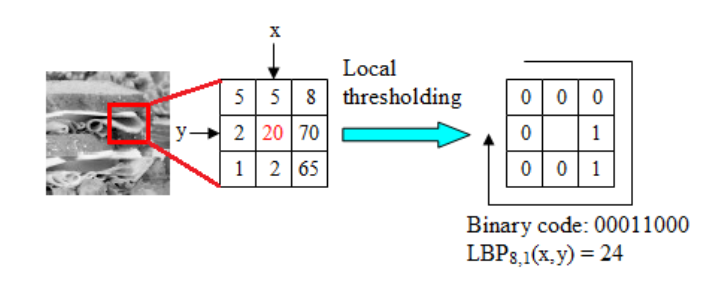
\includegraphics[scale=0.55]{img/lbp}
    \caption{Illustration of the LBP descriptor's process}
    \label{fig:lbp_process}
\end{figure}

We adopt the following notation. Given a pixel $c = (x_c, y_c)$, the value of the $LBP$ code of $c$ is defined as:
$$LBP_{P, R} (x_c, y_c) = \sum_{p = 0}^{P - 1} s (g_p - g_c) 2^p$$
where:
\begin{itemize}
    \item $p$ is a neighbour pixel of $c$ and the distance from $p$ to $c$ does not exceed $R$. Thus, $R$ is the radius of a circle centered in $c$ and $P$ is the numbered of sampled points.
    \item $g_p$ and $g_c$ are the gray values (intensities) of $p$ and $c$
    \item $s(x)$ is the function defined as:
    \begin{equation}
    s(x) =
    \begin{cases}
    1 & \text{if $x \geq 0$}\\
    0 & \text{otherwise} \\
    \end{cases}
    \end{equation}
\end{itemize}

In Fig. \ref{fig:lbp_process}, $R$ and $P$ are 1 and 8 respectively.

The number of histograms bins for $LBP_{P, R}$ is $2^P$.

Lastly, it’s important that we consider the concept of LBP uniformity. A LBP is considered to be uniform if it has at most two 0-1 or 1-0 transitions. For example, the pattern 00001000  (2 transitions) and 10000000  (1 transition) are both considered to be uniform patterns since they contain at most two 0-1 and 1-0 transitions. The pattern 01010010 ) on the other hand is not considered a uniform pattern since it has six 0-1 or 1-0 transitions.

The number of uniform prototypes in a Local Binary Pattern is completely dependent on the number of points p. As the value of p increases, so will the dimensionality of your resulting histogram. Please refer to the original Ojala et al. paper for the full explanation on deriving the number of patterns and uniform patterns based on this value. However, for the time being simply keep in mind that given the number of points p in the LBP there are p + 1 uniform patterns. The final dimensionality of the histogram is thus p + 2, where the added entry tabulates all patterns that are not uniform.

\section{Color descriptor}

\subsection{Color histogram}

HSV channels: Hue, Saturation and Value.
It has been defined to be closer to the way human represents colours.
Hue and Saturation corresponds to the chromaticity of the colour, Value to the lightness.
As value is really dependant of the condition where the picture were taken, we don't use it for color histogram.

\subsection{Color moments}

\subsection{The first two moments}

For a discrete random variable $X$, the first two moments are defined as:
\begin{itemize}
    \item \textbf{Expected value}: $$\E \left[ X \right] = \mu = \sum_{i = 1}^{n} p_i x_i $$
    \item \textbf{Variance}:  $$ \Var (X)= \E \left[ (X - \E \left[ X \right] )^2 \right] =\sum _{i=1}^{n} p_i (x_{i} - \mu )^{2} $$
\end{itemize}

\subsection{Hu moments}

\subsubsection{Raw moments}

For a two-dimensional continuous function f(x,y) the moment (sometimes called \enquote{raw moment}) of (p + q)th order is defined as: 
$$M_{pq}=\int \limits _{-\infty }^{\infty }\int \limits _{-\infty }^{\infty }x^{p}y^{q}f(x,y) dx dy $$
for $p$ and $q \in \N $

\subsubsection{Central moments}

And the central moments are :
$$\mu_{pq}=\int \limits_{-\infty }^{\infty }\int \limits _{-\infty}^{\infty} (x- \bar{x})^{p}(y - \bar{y})^{q} f(x,y) dx dy $$
with $\bar{x}=\frac{M_{10}}{M_{00}}$ and $\bar{y}=\frac{M_{01}}{M_{00}}$

\subsubsection{Normalized central moments}

The normalized central moments are:
$$\eta_{ij}=\frac{\mu _{ij}}{\mu_{00}^{\gamma}}$$
where $\gamma = 1 + \frac{I + j}{2}$ for $i + j \geq 2$

\subsubsection{Definition of the Hu moments}

On the base of those Moments, Hu in \cite{Hu1962} introduced 7 Moments which are invariant for translation, rotation and resizing:
\begin{align*}
    I_{1} = & \eta _{20}+\eta _{02} \\
    I_{2} = & (\eta _{20}-\eta _{02})^{2}+4\eta _{11}^{2} \\
    I_{3} = & (\eta _{30}-3\eta _{12})^{2}+(3\eta _{21}-\eta _{03})^{2} \\
    I_{4} = & (\eta _{30}+\eta _{12})^{2}+(\eta _{21}+\eta _{03})^{2} \\
    \begin{split}
        I_{5} = & (\eta _{30}-3\eta _{12})(\eta _{30}+\eta _{12})[(\eta _{30}+\eta _{12})^{2}-3(\eta _{21}+\eta _{03})^{2}] \\
        & +(3\eta _{21}-\eta _{03})(\eta _{21}+\eta _{03})[3(\eta _{30}+\eta _{12})^{2} -(\eta _{21}+\eta _{03})^{2}]
    \end{split} \\
    I_{6} = & (\eta _{20}-\eta _{02})[(\eta _{30}+\eta _{12})^{2}-(\eta _{21}+\eta _{03})^{2}]+4\eta _{11}(\eta _{30}+\eta _{12})(\eta _{21}+\eta _{03}) \\
    \begin{split}
        I_{7} = & (3\eta _{21}-\eta _{03})(\eta _{30}+\eta _{12})[(\eta _{30}+\eta _{12})^{2}-3(\eta _{21}+\eta _{03})^{2}] \\
        & - (\eta _{30}-3\eta _{12})(\eta _{21}+\eta _{03})[3(\eta _{30}+\eta _{12})^{2}-(\eta _{21}+\eta _{03})^{2}]
    \end{split} \\
\end{align*}

\section{Bag-of-Words}
\subsection{Process}

\textbf{Bag-of-Words} \textit{BoW}, also called Bag of features, is a feature descriptor method inspired by information retrieval from textual documents.

As illustrated in Fig. \ref{fig:bow_process}, the main steps are:
\begin{itemize}
    \item On each picture, keypoints are detected (in my case, I use a dense grid).
    \item For every keypoint, we describe it, SIFT (scale invariant feature transform).
    \item We generate the fix number of visual words that compose our codebook.
    \item We express each image as an histogram of these words' appearance.
\end{itemize}

\begin{figure}
    \centering
    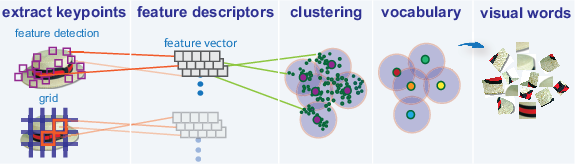
\includegraphics[scale=0.9]{img/bow.png}
    \caption{Illustration of the Bag-Of-Visual-Words model}
    \label{fig:bow_process}
\end{figure}

cite who use it first?

overall process

Sift

Surf

Feature detection
- can use sift or surf
- dense grid (cite why it is better)

Descriptor

clustering
- k means
